\chapter{ SIFT en GPU}

La correcta paralelización de un algoritmo no es nada trivial. Después de el capitulo anterior, al ver todas las ventajas que tenemos en los GPU`s podríamos decir que son la solución a todo, tristemente no lo son, existen algoritmos que por la estructura del programa y forma de ejecutar el proceso, no se podrían paralelizar. Para saber como analizar si un algoritmo es paralelizable primero debemos dar una definición de que es un programa paralelo:

\begin{center}
\textit{"Programa paralelo es la especificación de dos o mas procesos simultáneos que cooperan entre si con un fin en común"}
\end{center}

Podemos sacar dos aspectos importantes de esta definición el primero es la comunicación, los procesos deben poder compartir información  para poder trabajar simultáneamente sobre un mismo problema; el segundo es la sincronización, es simplemente como organizar a los procesos para que mientras realizan su parte de trabajo sin que se interfieran entre ellos.
Entonces tenemos que cambiar la forma en que programamos, ahora no solo pensaremos como llegar a un objetivo paso a paso, sino  que debemos pensar como muchos procesos trabajaran juntos para alcanzar un objetivo, esto inmediatamente me da la idea de repartir o dividir el trabajo entre todos ellos. Así que para realizar la labor de paralelizar el algoritmo debemos analizar básicamente tres casos de paralelismo:
 
\begin{itemize}
 
	\item \textit{Funcional}: Aquí lo que se divide es el algoritmo, buscamos pasos en el algoritmo que no dependan de otra parte del mismo y los ponemos a ejecutarse simultáneamente en diferentes 		procesos. Requiere de sincronizan muy cuidadosamente para que las diferentes partes de el algoritmo no interfieran entre si. 
	
	\begin{figure}[h]
			\centering
				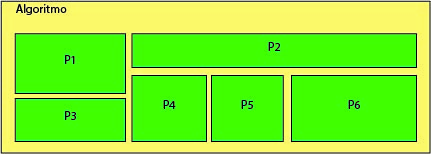
\includegraphics[scale=0.7]{img/funcional.jpg}
			\caption{Todos los procesos son partes diferentes del algoritmo}
	\end{figure}

	\item \textit{Dominio}: Se repartirán los datos en los múltiples procesos los cuales tienen una especificación idéntica. El sincronizan es sencillo en este caso, pero aun así hay que presentar atención ya que podríamos corromper información.
	\begin{figure}[h]
			\centering
				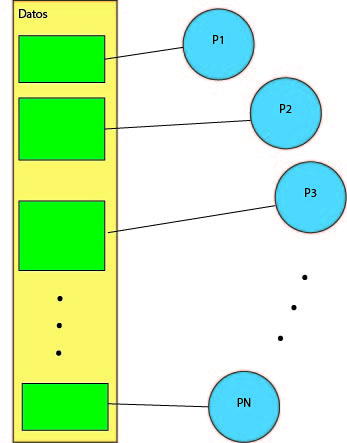
\includegraphics[scale=0.6]{img/dominio.jpg}
			\caption{Todos los procesos tienen la misma especificación }
	\end{figure}

	\item 	\textit{Actividad}: Es una combinación de los dos puntos anteriores.
\end{itemize}

Ahora que tenemos el algoritmo y las herramienta para mejorar su rendimiento por medio de la paraleización. Veremos como analizamos las partes de SIFT para de esta manera adaptarlo al modelo de programación de CUDA.
\pagebreak
\section{Análisis de SIFT para su Paralelización en GPU}

En esta sección se describe como se comunicaran y sincronizar los procesos, así como la estructura que tomara el algoritmo de SIFT, para poder paralelizarlo con CUDA. 

Primero dividiremos en 6 partes el algoritmo de SIFT, como se muuestra en la figura 4-3 , estas partes no se ejecutaran simultáneamente, es solo que el algoritmo es bastante largo y al separarlo en estas partes podemos simplificarlo en diferentes kernels, que tendrán una secuencia de ejecución. 

\begin{figure}[h]
			\centering
				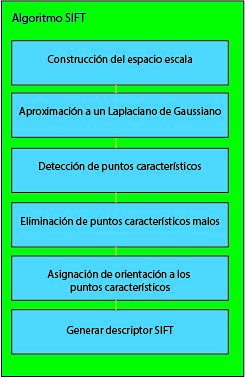
\includegraphics[scale=1]{img/SIFTdiv.jpg}
			\caption{División del algoritmo SIFT a paralelizar}
\end{figure}



Los kernels de las diferentes partes del algoritmo tienen una estructura en común, básicamente todos tiene como entrada una o mas imágenes, las cuales serán de solo lectura, y obtendremos una imagen o varias de salida. Cada proceso tendrá una sección de la imagen de tamaño  $N \times N$, la cual puede estar traslapada con la de algún otro proceso, pero esta área no requiere de sincronizar entre procesos ya que solo sera para obtener datos, para procesarlos.En la imagen de salida el proceso se le sera asignado solo un pixel de la imagen para escribir, como se puede mostrar en la figura 4-4 las zonas del P1 y P2 están traslapadas y en la imagen de salida, que es como si tuviera un zoom a los pixeles, no escriben en otro que no sea su pixel. Los procesos que se ejecutan sobre la imagen tienen la misma especificación, lo que quiere decir que lo que estamos repartiendo entre los múltiples procesos, serán los datos de entrada, con lo cual estaremos en la categoría de paralelismo de \textit{dominio}.


\begin{figure}[h]
			\centering
				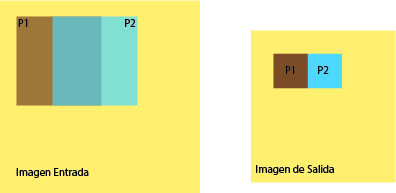
\includegraphics[scale=1]{img/prosImg.jpg}
			\caption{Proceso general de los kenels }
\end{figure}


Cada uno de los kernels serán ejecutados múltiples veces, este trabajo sera desempeñado por el anfitrión (CPU) de forma secuencial, esto es importante ya que cada uno de estos kernels es lanzado sin importar que el anterior acabara de ejecutarse, si múltiples kernels son lanzados y tiene la misma especificación pero trabajan con diferentes secciones de los datos no existe problema. Pero si el anfitrión llegara a lanzar un kernel que tiene una especificación diferente a la de un banco de kernels iguales lanzados anteriormente y estos no han finalizado puede existir riesgo de corromper los datos. Entonces debemos de sincronizar , como se puede ver en la figura 4-5, al  dispositivo (GPU) con el anfitrión (CPU) para evitar caer en este tipo de errores.

\begin{figure}[h]
			\centering
				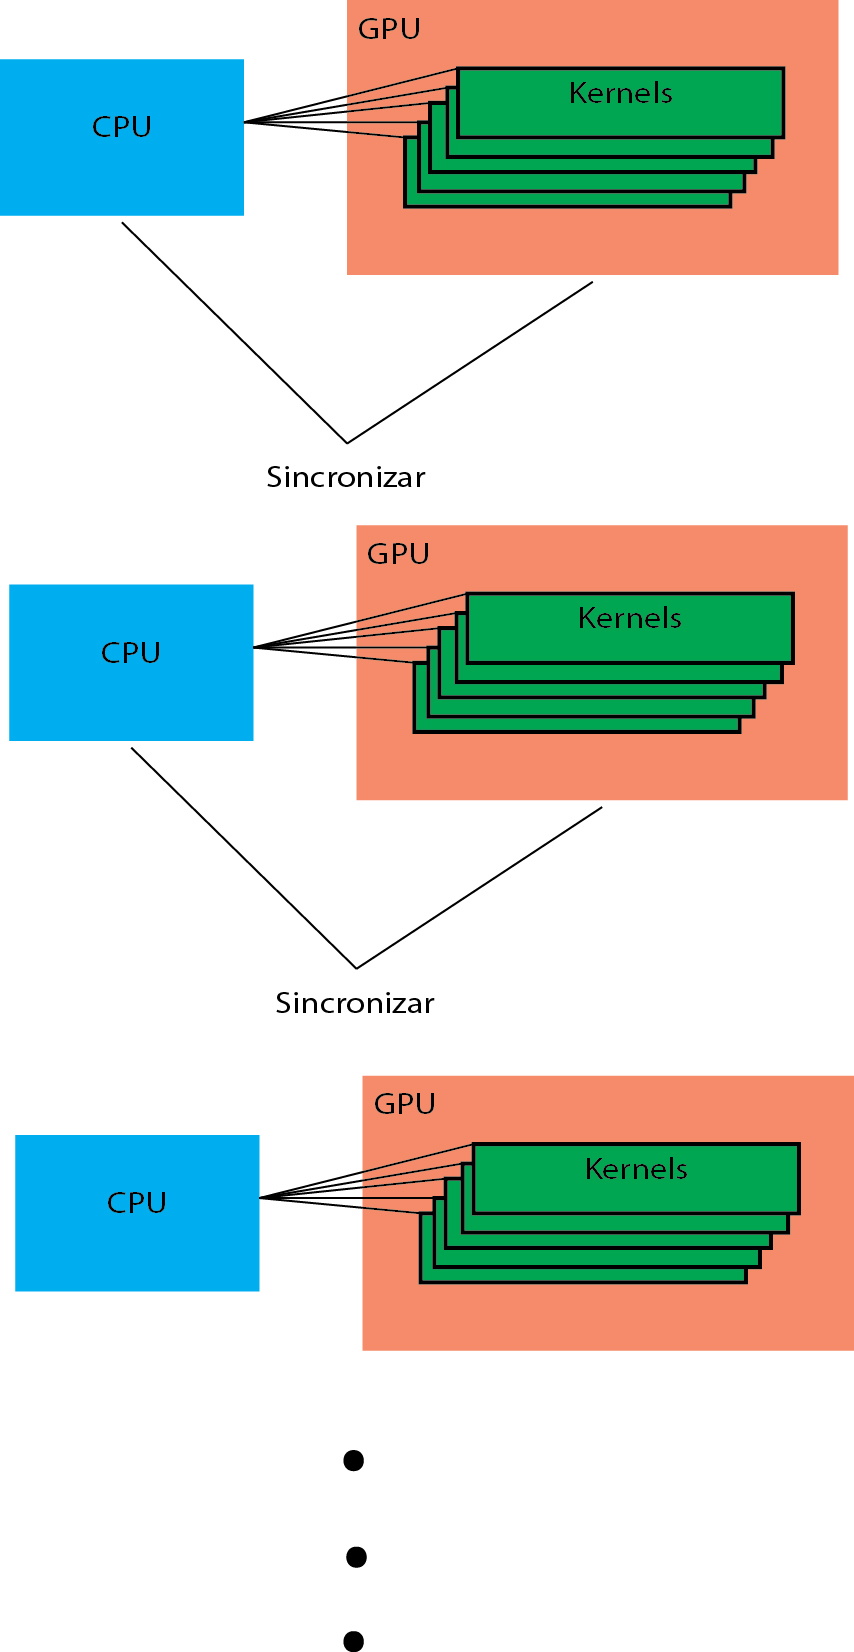
\includegraphics[scale=1]{img/lanzamiento.jpg}
			\caption{Lanzamiento de Kernels }
\end{figure}

\pagebreak
\section{Implementación}
hola



